The following subsections describe the impact of the different parameters the \lstinline|eStatics| package accepts on the computational performance. The impact can be measured several ways, for example by the time the program takes to finish computing or the number of iterations that were required to reach a certain level of accuracy. 

The \lstinline|eStatics| package accepts the following parameters:
\begin{itemize}
	\item The bitmap representing the system being computed
	\item The potential corresponding to each colour in the bitmap
	\item The maximum iterations the program is allowed to run for
	\item The relaxation level
	\item The desired convergence level
\end{itemize}

Most of the data used for the following graphs was gathered from computations done on System A, if not stated otherwise.

\subsubsection{Iterations}
The number of iterations the program is allowed to run for obviously has a great impact on the length of the computation, unless an accepted convergence level is reached before it. The number of iterations allowed also affects the accuracy of the final approximation, for if the program doesn't reach a predefined convergence level, it will continue converging in on the solution. 

Figure \ref{fig:iterations_vs_accuracy_abs} shows the accuracy of the final approximation compared to the number of iterations the program was run for. The accuracy converges to an absolute error of about $0.5$ per point compared to the analytic solution.

\begin{figure}[h!]
\centering
\setlength\fboxsep{0pt}
\setlength\fboxrule{0.5pt}
\fbox{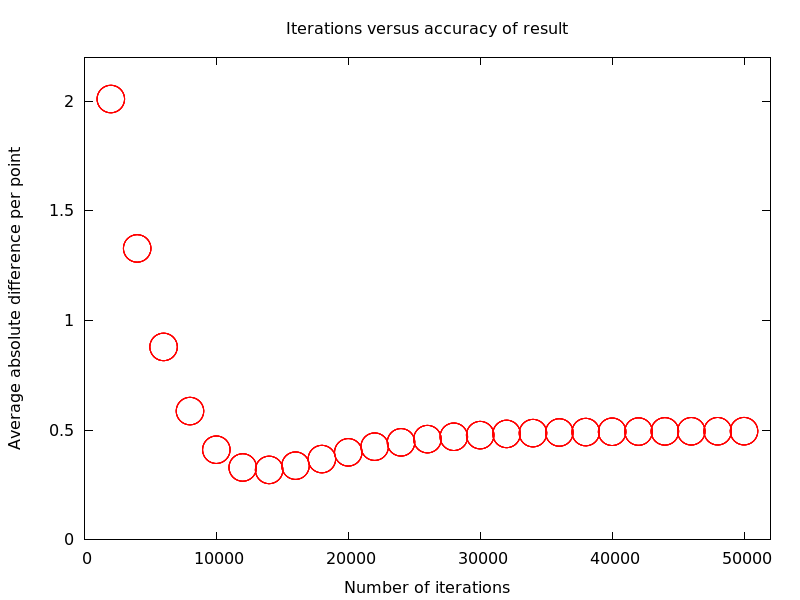
\includegraphics[width=0.95\textwidth, trim = 0mm 0mm 0mm 0mm, clip]{images/iterations_vs_accuracy_abs.png}} % change trim as required to eliminate unnecessary whitespace. trim: left bottom right top
\label{fig:iterations_vs_accuracy}
\caption{Figure showing the average absolute error per point for a given number of iterations calculated.}
\end{figure}

\subsubsection{Convergence}
The predefined convergence level affects the accuracy of the final solution greatly. Most of the error in the computation comes from around the boundaries or edges defined in the bitmap images. A very low desired convergence level is going to require more iterations by the program to reach it, while a high desired convergence may require next to no iterations at all. 

A typical desired convergence level would be somewhere between $10^{-6}$ and $10^{-9}$. This means that successive computations of the same point need to differ by less than $10^{-6}$ to $10^{-9}$ in order for the point to be locked and deemed to have converged at the solution. Setting a lower desired convergence level thus leads to a more precise solution. 

As can be seen on figure \ref{fig:convergence_accuracy}, the numerical approximation converges to an average absolute error of $0.496570$ per point as the level of desired convergence decreases. The $~0.5$ error per point is mostly due to systematic errors from around the boundaries as those are not changed by the numerical method. 

\begin{figure}[h!]
\centering
\setlength\fboxsep{0pt}
\setlength\fboxrule{0.5pt}
\fbox{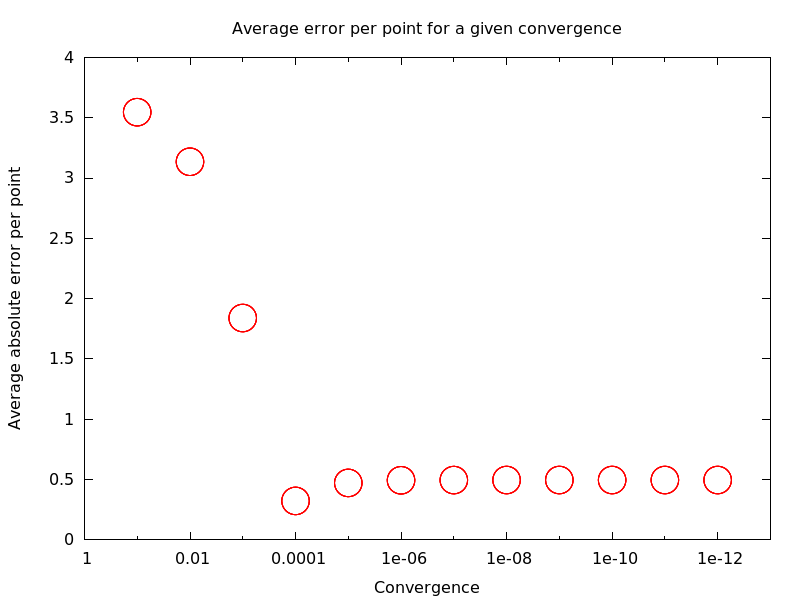
\includegraphics[width=0.95\textwidth, trim = 0mm 0mm 0mm 0mm, clip]{images/convergence_accuracy.png}} % change trim as required to eliminate unnecessary whitespace. trim: left bottom right top
\label{fig:convergence_accuracy}
\caption{Figure showing the average absolute error per point for a given desired convergence.}
\end{figure}

\subsubsection{Relaxation level}
There exists an optimal relaxation level for each system. By plotting the required iterations for different relaxation levels between $1.9$ and $2.0$, as in figure \ref{fig:relax_narrow}, the optimal value is determined to be about $1.9775$, which reduces the number of required iterations to reach a convergence level of $10^{-6}$ from over $42000$ to just $670$, a difference of nearly two orders of magnitude. 

\begin{figure}[h!]
\centering
\setlength\fboxsep{0pt}
\setlength\fboxrule{0.5pt}
\fbox{\includegraphics[width=0.95\textwidth, trim = 0mm 0mm 0mm 0mm, clip]{images/relax_narrow.png}} % change trim as required to eliminate unnecessary whitespace. trim: left bottom right top
\label{fig:relax_narrow}
\caption{Figure showing how the number of iterations required to solve System A changes as the relaxation level approaches the optimal value.}
\end{figure}

The accuracy of the solution is not affected negatively by the reduced number of iterations, as the average absolute difference per point is $0.496569$, almost precisely the same as what the solution tends to as the desired convergence tends to zero.

For system C, the optimal relaxation level was determined to be $1.9850$, as can be seen in figures \ref{fig:sysC_relax_wide} and \ref{fig:sysC_relax_narrow}. The program required only $973$ iterations to reach a convergence level of $10^{-6}$ with relaxation level $1.9850$, while with relaxation level of $1.0$, it took over $99000$ iterations. Again, the improvement is nearly two orders of magnitude.

\begin{figure}[h!]
\centering
\setlength\fboxsep{0pt}
\setlength\fboxrule{0.5pt}
\fbox{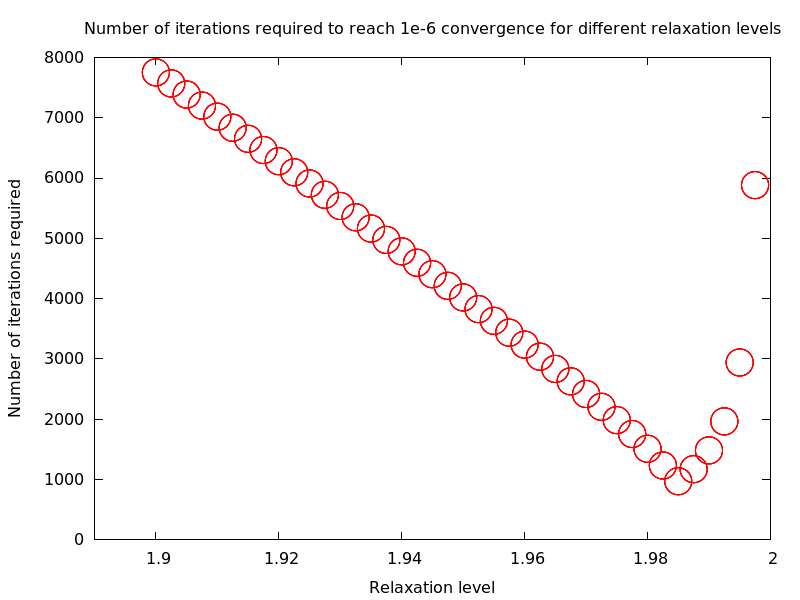
\includegraphics[width=0.95\textwidth, trim = 0mm 0mm 0mm 0mm, clip]{images/sysC_relax_narrow.png}} % change trim as required to eliminate unnecessary whitespace. trim: left bottom right top
\label{fig:sysC_relax_narrow}
\caption{Figure showing how the number of iterations required to solve System C changes as the relaxation level approaches the optimal value.}
\end{figure}

\subsubsection{Multithreading}
Multithreading can have a great impact on the time taken to run a program. Figure \ref{fig:multiple_multithreads} shows the impact on computation time when using different number of threads on \lstinline|eStatics|. The difference becomes more and more substantial when each thread has more work to do, so the multithreading process is ideal for computing larger grids.

\begin{figure}[h!]
\centering
\setlength\fboxsep{0pt}
\setlength\fboxrule{0.5pt}
\fbox{\includegraphics[width=0.95\textwidth, trim = 0mm 0mm 0mm 0mm, clip]{images/multiple_multithreads.png}} % change trim as required to eliminate unnecessary whitespace. trim: left bottom right top
\label{fig:multiple_multithreads}
\caption{Comparing the time required for a varying number of iterations with 1-8 threads.}
\end{figure}
